\chapter{Background}
\label{chap:background}
	\textit{In this chapter, we introduce the foundation knowledge of the thesis, including the history and definition of Blockchain Technology, Cryptocurrency, 
	Hierarchical Deterministic Wallet (HD Wallet) and Cryptography}
\minitoc

\section{Blockchain Technology}

\subsection{History and Definition}

Blockchains are immutable digital ledger systems implemented in a distributed fashion (i.e., without a central repository) and usually without a central authority.
The definition of blockchain was introduced to the world by a person (or a group of people) under the name Satoshi Nakamoto on October 31, 2008. 
It was applied to enable the emergence of a "purely peer-to-peer (no financial institution or third party) electronic cash" named Bitcoin where transactions take place in a distributed system.
In fact, Satoshi did not invent blockchain, and Bitcoin blockchain is not the first chain that ever created. 
Back in 1991, cryptographers Stuart Haber and Scott Stornetta published a whitepaper "How to Time-Stamp a Digital Document" in the Journal of Cryptography. 
Their goal is to digital time-stamping of documents so that it is infeasible for a user either to back-date or to a forward-date digital document, even with the collusion of a time-stamping service. 
The technology is called a blockchain because the distributed electronic ledger stores items of data in time-stamped digital groups called blocks. Each block includes an alphanumeric code called a "hash" summing up its data. The hash of each completed block also appears in the next one in the chain, which means that to alter one block you would have to alter all the ones connected to it. These cryptographic dominos function together to protect against tampering or fraud.
Base on this theory, the longest-running blockchain, started in 1995, also by Haber and Stornetta, publishes the weekly summary hash value every week in the New York Times (\autoref{fig:first_blockchain}) and still running strong today. 

\begin{figure}[h!]
	\centering
	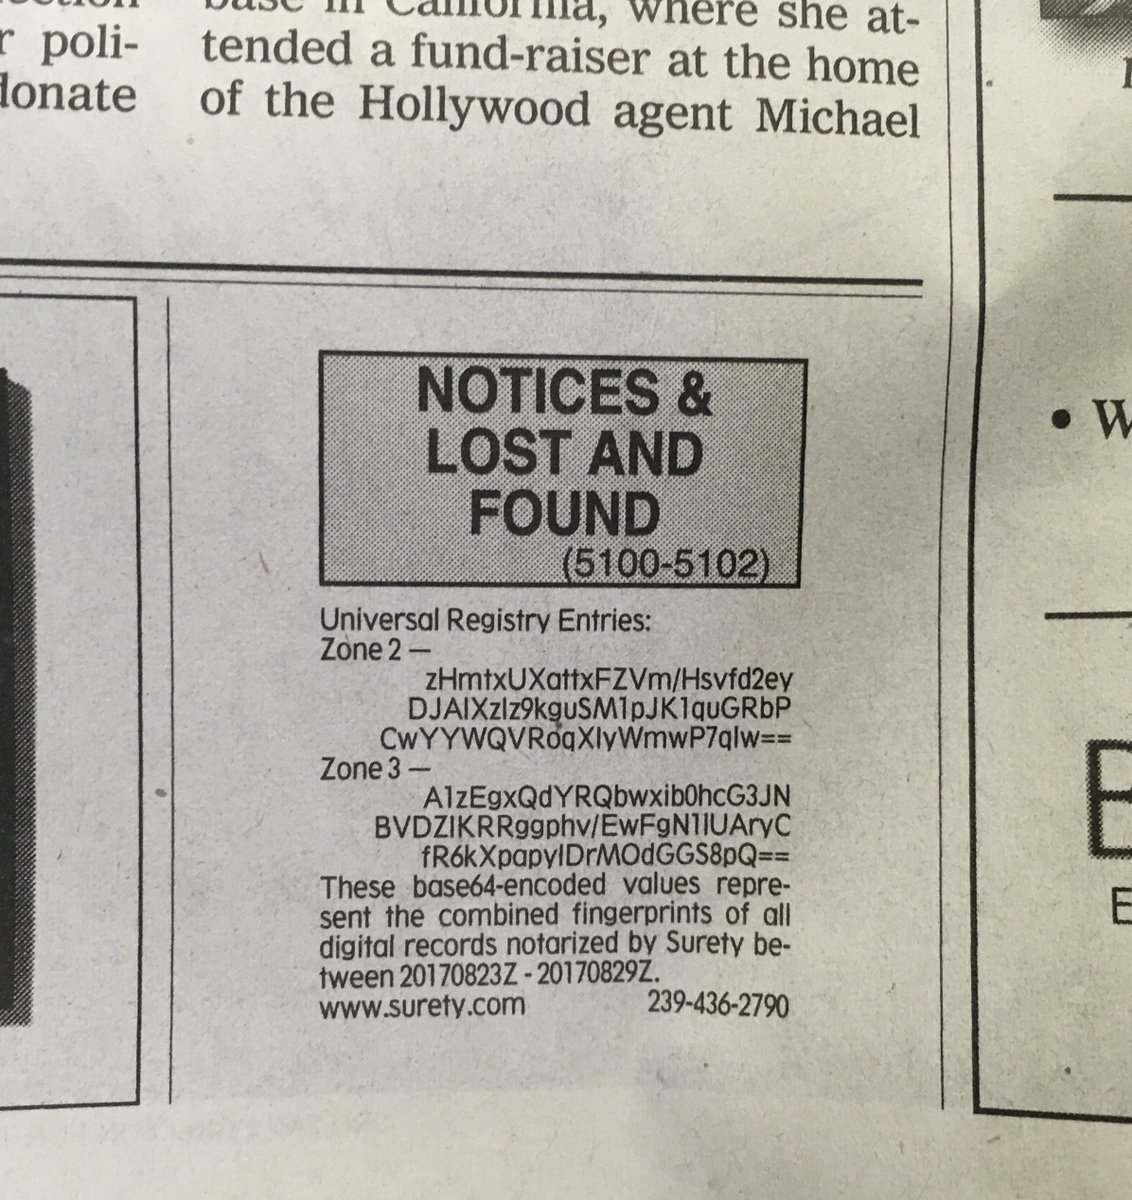
\includegraphics[width=.35\textwidth]{images/Widely_Witnessed_Values.jpg}
	\caption[Widely-Witnessed Values of Surety, a weekly summary (hash) of documents]{Weekly summary hash value in The New York Times}
	\label{fig:first_blockchain}
\end{figure}

% The math behind blockchain and its complex system architecture make it challenging to understand. 
But the word "blockchain" or "block" and "chain" wasn't use back then. 
Only it become known in Satoshi Nakamoto's Bitcoin paper in the term of "chain" of "blocks".
Later people combined the one-word "blockchain" in mainstream media publications such as Fortune, Forbes, and the Huffington Post as the technology gained greater interest and use. 
The comunity use that word for Nakamoto's invention.
Bound to emergence of Bitcoin and cryptocurrency, a concise description of blockchain technology is provided by NIST:

\begin{quote} 
	Blockchains are distributed digital ledgers of cryptographically signed transactions that are grouped into blocks. Each block is cryptographically linked to the previous one (making it tamper evident) after validation and undergoing a consensus decision. As new blocks are added, older blocks become more difficult to modify (creating tamper resistance). New blocks are replicated across copies of the ledger within the network, and any conflicts are resolved automatically using established rules.
\end{quote}

Blockchain technology comes handy in a wide range of areas - both ​financial and non-financial​. 
Non-Financial application opportunities are endless. 
We can envision putting proof of the existence of all legal documents, health records, and loyalty payments in the music industry, notary, private securities and marriage licenses in the blockchain. 
By storing the fingerprint of the digital asset instead of storing the digital asset itself, the anonymity or privacy objective can be achieved.
For the sake of our thesis, we will mainly focus on the original and surely the most popular application of blockchains - Cryptocurrency.

Cryptocurrencies are digital currencies that use blockchain technology to\autoref{fig:first_blockchain}) and still running strong today. 
record and secure every transaction. 
A cryptocurrency can be used as a digital form of cash that can be used to buy goods and services. 
It can be bought using one of several digital wallets or trading platforms, then digitally transferred upon purchase of an item, with the blockchain recording the transaction and the new owner. 
The appeal of cryptocurrencies is that everything is recorded in a public ledger and secured using cryptography, making an irrefutable, timestamped, and secure record of every payment.
The ledger displays user account balances and inter-user payments in a “currency” defined by the ledger itself and not necessarily in one of the traditional currencies. 
Nevertheless, cryptocurrency may be traded on the stock exchange and exchanged for traditional money, which makes it hard to distinguish between traditional currency and cryptocurrency and as official vs. non-official currency. 
The most widely recognized cryptocurrency system is Bitcoin.

We believe the "magic" that brings the above concept of digital currencies to reality, besides blockchain technology, is Nakamoto's proof-of-work consensus model.

\subsection{Blockchain Categorization and Generations}

Blockchain systems can be:
\begin{itemize}
	\item \emph{Permissioned blockchain}, where users publishing blocks must be authorized by some authority (be it centralized or decentralized). 
	Users of blockchain have to trust that entity or user who published blocks. 
	Permissioned blockchain networks may thus allow anyone to read the blockchain or they may restrict read access to authorized individuals. This maybe used by organizations that need more control over their blockchain.
	Some permissioned blockchain networks support the ability to selectively reveal transaction information based on a blockchain network users identity or credentials. 
	Some of famous permissioned blockchain applications are Ripple, which enables interbank transactions, or Sovrin, which is managed by financial institutions and is seeking to build a global decentralized identity system.
	
	\item \emph{Permissionless blockchain}, where service providers are not fixed and, in principle, anyone can start operating the service. For example, Bitcoin and the early versions of Ethereum.
	
\end{itemize}

% The blockchain is usually stored and managed in the form of a distributed ledger,
% with multiple parties keeping a copy of the ledger, which then implies the use of a
% handshake protocol between the components. However, also centralized blockchain
% system exist. The original and surely the most popular application of blockchains is
% cryptocurrency, where the ledger displays user account balances and inter-user payments
% in a “currency” defined by the ledger itself and not necessarily in one of the traditional
% currencies. Nevertheless, cryptocurrency may be traded on the stock exchange and
% exchanged for traditional money, which makes it hard to distinguish between traditional
% currency and cryptocurrency and as official vs. non-official currency. The most widely
% recognised cryptocurrency system is Bitcoin, which establishes and uses Bitcoins and
% Satoshis as currency.

% Most permissionless blockchain systems include an independent cryptocurrency. 
% The reason for that is that in the absence of an inter-operator contract, there are usually no other incentives to guarantee voluntary management of the Blockchain

Based on the intended audience, three generations of blockchains can be distinguished (Zhao et al., 2016):
\begin{itemize}

\item Blockchain 1.0 which includes applications enabling digital cryptocurrency transactions
\item Blockchain 2.0 which includes smart contracts and a set of applications extending beyond cryptocurrency transactions
\item Blockchain 3.0 which includes applications in areas beyond the previous two versions, such as government, health, science and IoT.

\end{itemize}

We are now developing blockchain 2.0 but our thesis just focus on cryptocurrency aspect.


\subsection{Bitcoin blockchain}
Bitcoin is the first application of blockchain and the most famous digital currency ever.
As mentioned above, Bitcoin was invented with the publication of a document entitled "Bitcoin: A peer-to-peer electronic cash system" in 2008 by Satoshi Nakamoto, mentioned as a purely P2P version of electronic cash would allow online payments to be sent directly from one party to another without going through a financial institution. 
The currency began to use in 2009 when its implementation was released as open-source software. 
The Bitcoin blockchain is considered to be a world-changing technology because in the first time in human history its solved the biggest problem of distributed system: The Byzantine General's Problem. 
We will talk about this in the Bitcoin game of theory and incentives section.

Bitcoin application is one of the permissionless blockchain.
It utilize well-known computer science mechanisms (linked lists, distributed networking) as well as cryptographic primitives (hashing, digital signatures, public/private keys) mixed with financial concepts (ledgers, games of theory) in high level. 
Base on the problems Bitcoin has solved, we examine by dividing it into 3 components:

\begin{itemize}
\item Secure and Prevent tempering the data

\begin{quote} 
	\emph{Hashes} - 
	Cryptographic hash functions (CHF) are used for hashing the content of a block, validating the integrity of data, reduce the size of the message or keys, generating a Bitcoin address. We will show detail at Section~\ref{sec:crypto_hash}.
	Hashing is a method of calculating a relatively unique fixed-size output (called a message digest, or just digest) for an input of nearly any size (e.g., a file, some text, or an image).
	Even one single bit change of input will result in a completely different output digest. 
	In Bitcoin and most blockchain technologies, SHA-256 (Secure Hash Algorithm with output size of 256 bits) appear the most. Many computer support hardware level for this algorithm.
	NIST specified this algorithm for SHA-256 in Federal Information Processing Standard (FIPS) 180-4 as it passed every properties of a cryptographic hashing.
	\autoref{fig:example_of_sha-256} is an example of SHA-256.

		\begin{figure}[h!]
			\centering
			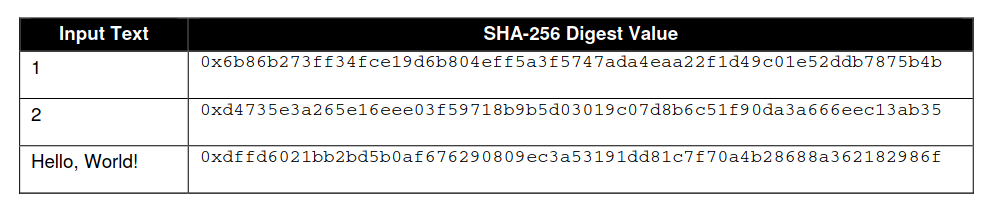
\includegraphics[width=1\textwidth]{images/example_of_sha-256.png}
			\caption[Example input and output of SHA-256 Digest Value]{Example I/O of SHA-256 Digest Value}
			\label{fig:example_of_sha-256}
		\end{figure}

	\bigbreak
	
	\emph{Public/Private Key} -	
	Asymmetric-key cryptography (or public-key cryptography) uses a pair of keys: a public key and a private key that are mathematically related. It could be infeasible to generate one key from the other.
	The private key is kept secret while the public key can be to everyone, both keys are hold inside user's Wallet, which we present in Section~\ref{sec:hd_wallet}.
	One can encrypt with a private key and then decrypt with the public key. 
	Alternately, one can encrypt with a public key and then decrypt with a private key.
	Bitcoin uses asymmetric-key cryptography to digitally sign transactions, verify signatures or in some cases, exchange the key.
	Asymmetric-key cryptography is discussed in Section~\ref{sec:asymmetric_cryptography}.
	Figure~\ref{fig:asymmetric_cryptography} briefly show message exchange usage of the asymmetric protocol.
	
	\begin{figure}[h!]
		\centering
		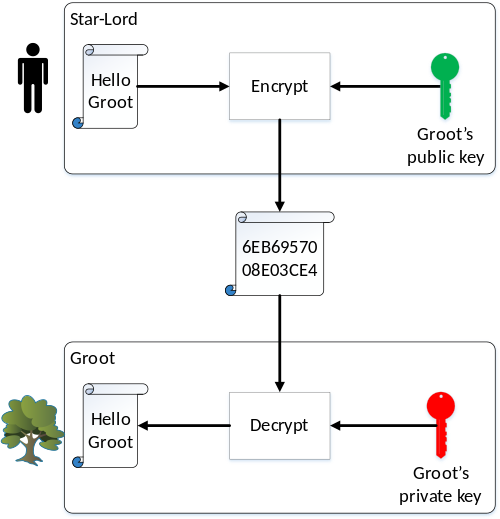
\includegraphics[width=0.4\textwidth]{images/asymmetric_cryptography.png}
		\caption[An example of concept of Asymmetric-key cryptography]{Sending private message using Asymmetric-key cryptography}
		\label{fig:asymmetric_cryptography}
	\end{figure}
	\bigbreak

	\emph{Transactions} - Transactions represent transfers of the cryptocurrencies between wallets in the system. 
	A transaction contains input and output. The inputs are usually a list of the digital assets to be transferred.
	Outputs are	the accounts that will be the recipients of the digital assets along with how much digital asset they will receive.   
	All values of in and out cannot be tampered.

	\begin{figure}[h!]
		\centering
		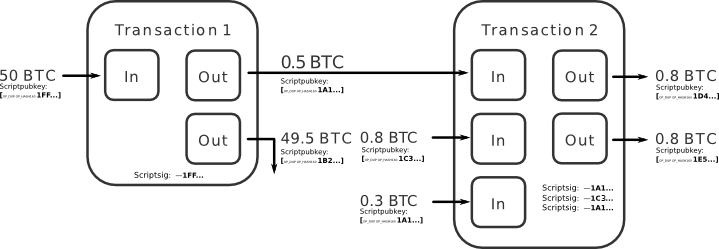
\includegraphics[width=0.7\textwidth]{images/transaction.png}
		\caption[An example of bitcoin transaction]{An example of bitcoin transaction}
		\label{fig:transaction}
	\end{figure}
	\bigbreak

	All transactions are broadcast to the network and usually begin to be confirmed within 10-20 minutes, through a process called \emph{mining}.
	Transactions are typically digitally signed by the sender’s associated private key and can be verified using the associated public key.

	\bigbreak

	\emph{Ledgers} - 
	A ledger is a collection of cryptographic transactions. 
	Bitcoin ledgers are distributed, the blockchain holds all accepted transactions within its ledgers. Every user can maintain their own copy of the ledger.
	Whenever new full nodes join the blockchain network, they reach out to discover other full nodes and request a full copy of the blockchain network’s ledger, making loss or destruction of the ledger difficult.
	\bigbreak
	
	The network utilizes cryptographic mechanisms such as digital signatures and cryptographic hash functions to provide tamper-evident and tamper-resistant ledgers.
	Due to the public distributed network, the Bitcoin blockchain is harder to attack. There is nothing to steal because everything is distributed. If one individual node got taken down, the network will still be running. 
	If targeting the blockchain itself, the attackers will face resistance from the honest nodes present in the system. 
	\bigbreak

	\emph{Blocks} -	
	Transactions, after sent to the network (by wallets, web applications, etc.), will be, if accepted, added to a block that is published by a chosen node. 
	Bitcoin blocks include block header and block data.
	Figure~\ref{fig:block_component} show basic component of a block.
	Block header contains version, previous block header’s hash value (prevBlockHash), a hash representation of the block data (usual Merkle tree* hash), a timestamp, size of the block (bits), a \emph{nonce}.
	The \emph{nonce} value is manipulated by the publishing node to solve the hash puzzle (see Section~\ref{subsec:game_theory})
	Block data contains a list of transactions and ledger events. Some include other data.
	\pagebreak

	\begin{figure}[h!]
		\centering
		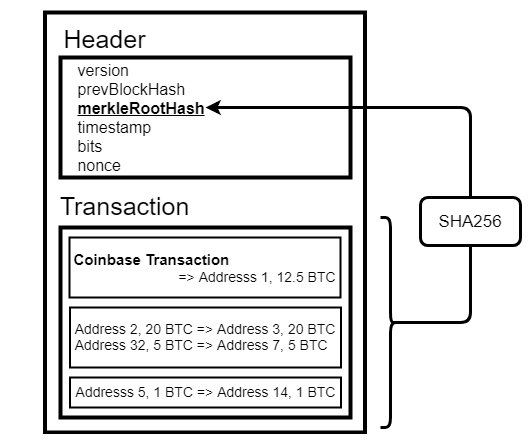
\includegraphics[width=0.6\textwidth]{images/block_component.jpg}
		\caption[Components of Bitcoin block]{Components of Bitcoin block}
		\label{fig:block_component}
	\end{figure}

	\emph{Chain of Blocks} - 
	Blocks are chained together through each block containing the hash digest of the previous block’s header, thus forming the blockchain.
	If one of the previous blocks were changed, it would result in a different hash.
	This makes it possible to easily detect and reject altered blocks

	\begin{figure}[h!]
		\centering
		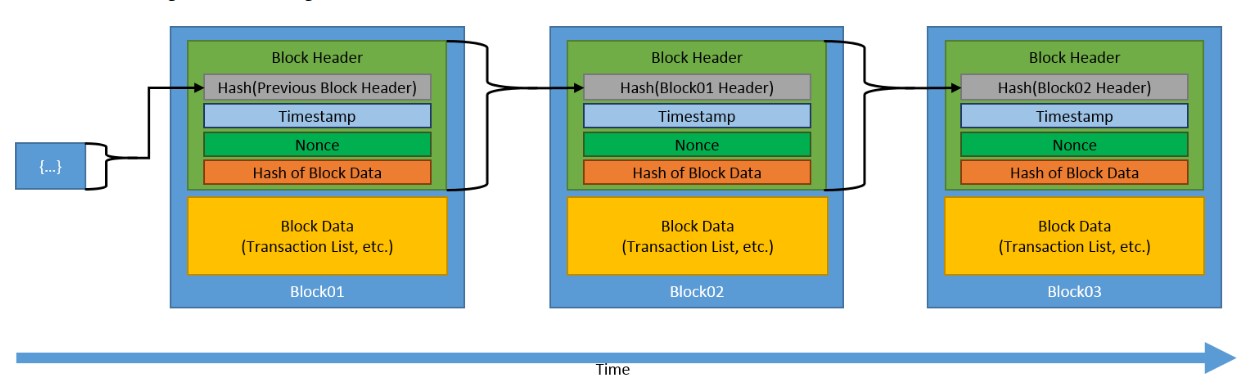
\includegraphics[width=1\textwidth]{images/chain_of_block.png}
		\caption[Components of Bitcoin block]{Components of Bitcoin block}
		\label{fig:chain_of_block}
	\end{figure}


\end{quote}

\item Game of theory and Incentives
\label{subsec:game_theory}

\begin{quote} 
	\emph{Hashes} - 
	Cryptographic hash functions (CHF) are used for hashing the content of a block, validating the integrity of data, reduce the size of the message or keys, generating a Bitcoin address. We will show detail at Section~\ref{sec:crypto_hash}.
	Hashing is a method of calculating a relatively unique fixed-size output (called a message digest, or just digest) for an input of nearly any size (e.g., a file, some text, or an image).
	Even one single bit change of input will result in a completely different output digest. 


\end{quote}
\item Communication Network

\begin{quote} 
	\emph{Hashes} - 
	Cryptographic hash functions (CHF) are used for hashing the content of a block, validating the integrity of data, reduce the size of the message or keys, generating a Bitcoin address. We will show detail at Section~\ref{sec:crypto_hash}.
	Hashing is a method of calculating a relatively unique fixed-size output (called a message digest, or just digest) for an input of nearly any size (e.g., a file, some text, or an image).
	Even one single bit change of input will result in a completely different output digest. 

\end{quote}

\end{itemize}



\section{HD Wallet}
\label{sec:hd_wallet}



\subsection{Category}

\subsection{Coins}

\subsection{Wallet structure}

\section{Cryptography}

\subsection{Cryptographic hash}
\label{sec:crypto_hash}

\subsection{Asymmetric-key cryptography}
\label{sec:asymmetric_cryptography}

\subsubsection{Diffie-Hellman algorithm}

\subsubsection{RSA Cryptography}

\subsubsection{EC Cryptography}

\subsection{Twisted-Edward curve and Ed25519}

\subsection{Key derivation function}
